\section{Paper-specific project}

\subsection{Data}
The datasets used in \cite{lewin2021sars} and \cite{lewin2022seroprevalence} together can be viewed as one for a serial COVID-19 seroprevalence study in Quebec, Canada. \\
\newline $ $
The first dataset contains numbers of antibody-positive samples as well as total number of samples for each region in Quebec (Montreal-Laval, surrounding Montreal-Laval, and other regions). These samples are collected relatively early on in the pandemic, from May 25 to July 9, 2020. The second dataset follows the same structure, but contains samples collected between January 25 and Mar 11, 2021. \\
\newline $ $
In addition, \cite{lewin2022seroprevalence} also contains results from a seroreversion substudy. Namely, we also have the number of antibody-positive samples from 2020 that remained positive in 2021. \\
\newline $ $
Note that in the second study, the count of antibody-positive samples are available at a finer scale (each of Montreal-Laval, surrounding Montreal-Laval, and other regions are broken down into smaller regions), this is not the case for \cite{lewin2021sars}. Therefore the analysis will only be conducted at the bigger regional level.

\begin{table}[]
\centering
\label{tab:dat}
\begin{tabular}{c|cc|cc|cc}
                           & \multicolumn{2}{c}{\textbf{Phase I}} & \multicolumn{2}{c}{\textbf{Phase II (unvaccinated)}} & \multicolumn{2}{c}{\textbf{Seroreversion substudy}}\\
                           & reactive      & tested      & reactive              & tested      & reactive              & tested        \\
                           \hline
Montreal-Laval             & 90            & 3061        & 48                    & 1925      & - & -          \\
Surrounding Montreal-Laval & 48            & 1925        & 128                   & 1422   & - & -             \\
Other                      & 35            & 2705        & 372                   & 4304          & - & -      \\
\hline
Total                      & 173           & 7691        & 715                   & 7304          &    32 & 109  
\end{tabular}
\caption{Seroprevalence data from \cite{lewin2021sars} and \cite{lewin2022seroprevalence}.}
\end{table}

\subsection{Project Idea}
We can apply the approach in \cite{meyer2022adjusting} to the two datasets in \cite{lewin2021sars} and \cite{lewin2022seroprevalence} in one coherent Bayesian model that accounts for seroreversion. \\
\newline $ $
Let $S_{ij}$ denote the true seroprevalence in study $i$ and region $j$ ($i=1$ and $i=2$ correspond to first and second study, $j=1,j=2$ and $j=3$ correspond to Montreal-Laval, surrounding Montreal-Laval, and other regions). Let $P_{ij}$ denote the observed seroprevalances. Let $Se, Sp, Sr$ denote sensitivity of test-kit, specificity of test-kit, as well as proportion of samples that has seroreverted (testing antibody-negative in 2021 but antibody-positive in 2020). Let $x_{ij}$ denote the total number of antibody-positive samples in region $j$ at study $i$, and $n_{ij}$ denote the total number of samples in region $j$ at study $i$. Finally, let $x_r$ and $n_r$ denote the total number of samples that seroreverted and the total number of samples in the seroreversion substudy. \\
\newline $ $
The model can then be written as
\[
P_{11} &= S_{11} \times Se + (1 - S_{11}) \times (1 - Sp)\\
P_{12} &= S_{12} \times Se + (1 - S_{12}) \times (1 - Sp)\\
P_{13} &= S_{13} \times Se + (1 - S_{13}) \times (1 - Sp)\\
P_{21} &= (S_{21} - Sr \times S_{11}) \times Se + (1 - (S_{21} - Sr \times S_{11})) \times (1 - Sp)\\
P_{22} &= (S_{22} - Sr \times S_{12}) \times Se + (1 - (S_{22} - Sr \times S_{12})) \times (1 - Sp)\\
P_{23} &= (S_{23} - Sr \times S_{13}) \times Se + (1 - (S_{23} - Sr \times S_{13})) \times (1 - Sp)\\
S_{11} &\sim \distBeta(\cdot, \cdot)\\
S_{12} &\sim \distBeta(\cdot, \cdot)\\
S_{13} &\sim \distBeta(\cdot, \cdot)\\
S_{21} &\sim \distBeta(\cdot, \cdot)_{\{ Sr \times S_{11} , 1 \}}\\
S_{22} &\sim \distBeta(\cdot, \cdot)_{\{ Sr \times S_{12} , 1 \}}\\
S_{23} &\sim \distBeta(\cdot, \cdot)_{\{ Sr \times S_{13} , 1 \}}\\
Se &\sim \distBeta(\cdot, \cdot)\\
Sp &\sim \distBeta(\cdot, \cdot)\\
Sr &\sim \distBeta(\cdot, \cdot)\\
L(P, S, Se, Sp, Sr \given X, N) &\propto \left(\prod_{i=1}^2\prod_{j=1}^3 P_{ij}^{x_{ij}} (1 - P_{ij})^{n_{ij} - x_{ij}}\right)\left( Sr^{x_r} (1-Sr^{n_r - x_r}) \right)
\]
Note that for observed seroprevalences in the first study, we adjust for test sensivitity and test specificity (Following the setup in \cite{meyer2022adjusting}. We'll likely use the same prior on $Se$ and $Sp$ here). For observed seroprevalences in the second study, we adjust for both test sensivitity and test specificity as well as seroreversion. Namely, we also include the proportion that have seroreverted since the first study using information from the seroreversion substudy. This combines the setup in \cite{lewin2022seroprevalence} and \cite{meyer2022adjusting}: we first substract the proportion that have seroreverted from the true seroprevalence and then adjust for test-kit performance. This is because the test-kit only has a chance at detecting antibodies if the subject has not seroreverted. To ensure we do not run into negative seroprevalence estimates, we truncate $S_{21}, S_{22}, S_{23}$ accordingly.\\
\newline $ $
Altogether, this can give us an estimate of the seroprevalance in Quebec, Canada in January to March 2021 adjusting for test-kit performance as well as seroreversion.\\
\newline $ $
We can compare the results from this above Bayesian model to those from \cite{lewin2022seroprevalence} (which is not Bayesian and does not account for test-kit performance) as well a frequentist equivalence of the above Bayesian model using the same data. We can use these results to check if the claims from \cite{lewin2022seroprevalence} still hold under this different dataset, as well as to explore potential reasons as to why they do or do not hold.\\
\newline $ $
It turns out that the intervals constructed from \cite{rosenberg2020cumulative} (the non-Bayesian analysis that \cite{meyer2022adjusting} compared to) is just by using the $95\%$ confidence interval endpoints for test sensitivity and specificity to correct for the true seroprevalence using $P = S \times Se + (1-S) \times (1-Sp)$.

\begin{table}[]
\centering
\label{tab:results}
\begin{tabular}{c|ccc}
                           & \multicolumn{3}{c}{\textbf{Raw result}}                                        \\
                           & mean                & lowerbound             & upperbound             \\
Montreal-Laval             & 0.136               & 0.120                  & 0.154                  \\
Surrounding Montreal-Laval & 0.090               & 0.076                  & 0.106                  \\
Other                      & 0.086               & 0.078                  & 0.095                  \\
\hline
                           & \multicolumn{3}{c}{\textbf{Adjusted for seroreversion}}                          \\
                           & mean                & lowerbound             & upperbound             \\
Montreal-Laval             & 0.145               & 0.125                  & 0.168                  \\
Surrounding Montreal-Laval & 0.097               & 0.080                  & 0.119                  \\
Other                      & 0.090               & 0.080                  & 0.102                  \\
\hline
                           & \multicolumn{3}{c}{\textbf{Adjusted for seroreversion and test-kit performance}} \\
                           & mean                & lowerbound             & upperbound             \\
Montreal-Laval             & 0.161               & 0.115                  & 0.177                  \\
Surrounding Montreal-Laval & 0.107               & 0.062                  & 0.120                  \\
Other                      & 0.100               & 0.056                  & 0.110                  \\
\hline
                           & \multicolumn{3}{c}{\textbf{Bayesian analysis adjusted for seroreversion and test-kit performance}}                                 \\
                           & median              & lowerbound             & upperbound             \\
Montreal-Laval             & 0.159               & 0.137                  & 0.183                  \\
Surrounding Montreal-Laval & 0.105               & 0.085                  & 0.125                  \\
Other                      & 0.096               & 0.082                  & 0.110                 
\end{tabular}
\caption{Summary of regional cumulative incidence point estimates and uncertainty intervals for all methods discussed.}
\end{table}

\captionsetup[subfigure]{labelformat=empty}
\begin{figure}[ht!]
\centering
\begin{subfigure}[b]{\columnwidth} 
    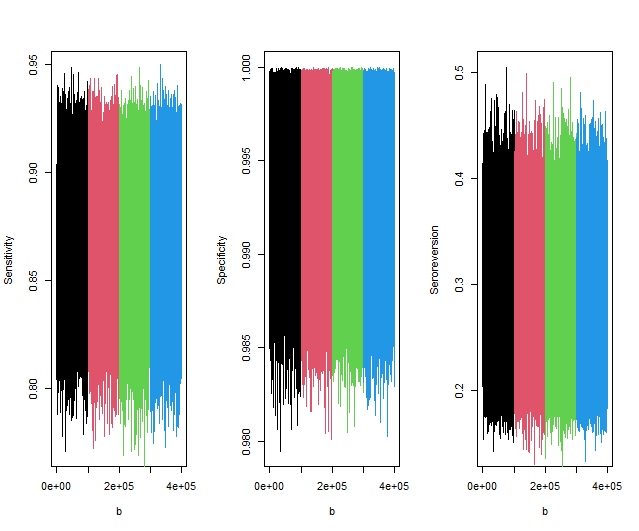
\includegraphics[width=\columnwidth]{../../plot/trace_global.png}
    \caption{Trace plots for test sensitivity ($se$), test specificity ($sp$), and seroreversion rate ($sr$).}
\end{subfigure}
\end{figure}

\captionsetup[subfigure]{labelformat=empty}
\begin{figure}[ht!]
\centering
\begin{subfigure}[b]{\columnwidth} 
    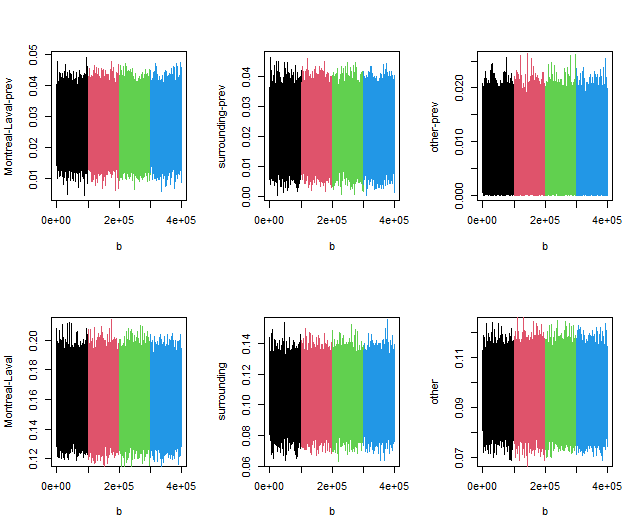
\includegraphics[width=\columnwidth]{../../plot/trace_regional.png}
    \caption{Trace plots for regional cumulative incidences. The first row correponds to cumulative incidences after Phase I of the study, and the second row correponds to cumulative incidences after Phase II of the study.}
\end{subfigure}
\end{figure}

\captionsetup[subfigure]{labelformat=empty}
\begin{figure}[ht!]
\centering
\begin{subfigure}[b]{\columnwidth} 
    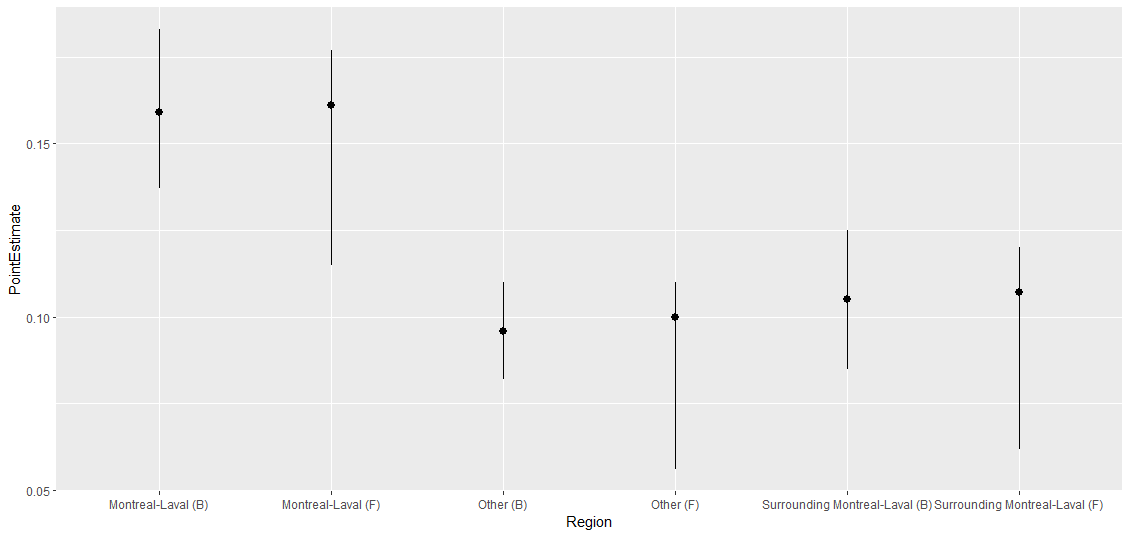
\includegraphics[width=\columnwidth]{../../plot/intervals.png}
    \caption{Comparison between uncertainty intervals for regional cumulative incidences between the Bayesian (B) and non-Bayesian (F) seroprevalence analyses, where both seroreversion and test-kit performance are accounted for.}
\end{subfigure}
\end{figure}